\documentclass[aspectratio=43]{beamer}

\usepackage[utf8]{inputenc}

\usepackage{amsfonts}
\usepackage{amsmath}
\usepackage{color}
\usepackage{listings}
\usepackage{tikz}
\usepackage{hyperref}

\usetheme{Rochester}
\usecolortheme{beaver}

\addtobeamertemplate{navigation symbols}{}{%
    \usebeamerfont{footline}%
    \usebeamercolor[fg]{footline}%
    \hspace{1em}%
    \insertframenumber/\inserttotalframenumber
}

\lstloadlanguages{C++}
    \lstset{%
        language={C++},
        basicstyle=\ttfamily,
        keywordstyle=\color{blue},
        showstringspaces=false,
        escapechar={§},
        escapeinside=||
    }

\newif\iftransitions
 \transitionstrue


\newif\iffast
% \fasttrue

\title{Taming Dynamic Memory}
\subtitle{An Introduction to Custom Allocators}
\author{Andreas Weis}
\institute{BMW AG}
\date{code::dive, November 7, 2018}
\titlegraphic{
\includegraphics[height=.2\textheight]{resources/codedive_logo.png}}

\iffalse
Taming dynamic memory - An introduction to custom allocators

Dynamic memory allocation is a feature that is often taken for granted. Most developers use some form of new or malloc every day, usually without worrying too much what goes on behind the scenes. But what about those situations where the built-in mechanisms are not good enough, be it for reasons of performance, safety, or due to restrictions of the target hardware? 

In this talk we will explore how custom allocators can be used to overcome those issues. We will explain how basic allocation techniques like pooling and monotonic allocation behave with regards to performance and reliability. We will take a look at some of the technical challenges behind allocators, like the different forms of alignment and the way that the standard library manages stateful allocators. And finally we will take a look at some popular allocator implementations and how to integrate them with a modern C++ codebase.

Audience
Developers that have never used a custom allocator before and don't know where to get started or don't understand what all the fuss is about.

Outline
- Scenarios in which the default allocator is not good enough
- Basic allocator toolbox: Stack, Monotonic, Pool, general-purpose; Explain the basic algorithm and pros & cons of each
- Popular open-source implementations of these
- Customization points for allocation in C++ and some popular third-party libraries; How they differ and how to bridge the gap.
- Using custom allocators for profiling, debugging and diagnostics
- Technical challenges when writing an allocator: Alignment, Strict aliasing, etc.
\fi

\begin{document}

\frame{\titlepage}

\iffalse %crop

\begin{frame}[fragile]
  \frametitle{About me}

  \begin{itemize}
    \setlength\itemsep{1.5em}

    \item \href{https://stackoverflow.com/users/577603/comicsansms}{
\includegraphics[height=.05\textheight]{resources/so-icon.png}} \href{https://github.com/ComicSansMS}{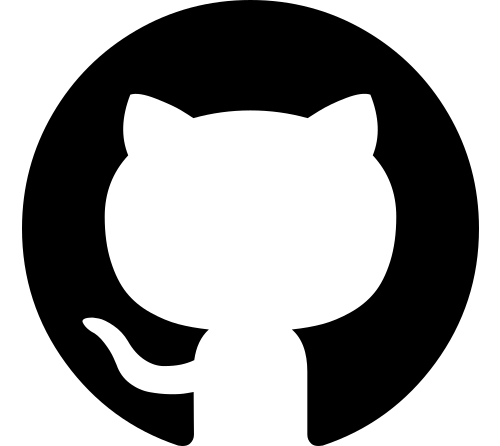
\includegraphics[height=.05\textheight]{resources/github-icon.png}} 
\includegraphics[height=.05\textheight]{resources/slack-icon.png} ComicSansMS

    \item \href{https://twitter.com/DerGhulbus/}{
\includegraphics[height=.05\textheight]{resources/twitter-icon.png} @DerGhulbus}

    \item 
\includegraphics[height=.05\textheight]{resources/meetup-icon.png} Co-organizer of the \href{https://www.meetup.com/MUCplusplus/}{Munich C++ User Group}

    \item Currently working as a Software Architect for BMW 
\includegraphics[height=.1\textheight]{resources/bmw_group.jpg}

  \end{itemize}
\end{frame}


\begin{frame}[fragile]
  \frametitle{General purpose allocator}
  \begin{center}
    \includegraphics<1>[width=.9\textwidth]{memgfx/gp_alloc_000.png}
    \includegraphics<2>[width=.9\textwidth]{memgfx/gp_alloc_010.png}
    \includegraphics<3>[width=.9\textwidth]{memgfx/gp_alloc_020.png}
%    \includegraphics<4>[width=.9\textwidth]{memgfx/gp_alloc_030.png}
    \includegraphics<4>[width=.9\textwidth]{memgfx/gp_alloc_040.png}
  \end{center}

    \begin{semiverbatim}
      \uncover<2->{\alert<0>{{\color{blue}auto} p1 = allocate(3);}}
      \uncover<3->{\alert<0>{{\color{blue}auto} p2 = allocate(4);}}
      \uncover<4->{\alert<0>{{\color{blue}auto} p3 = allocate(1);}}
      \uncover<4->{\alert<0>{{\color{blue}auto} p4 = allocate(3);}}
      \uncover<4->{\alert<0>{{\color{blue}auto} p5 = allocate(2);}}
    \end{semiverbatim}
\end{frame}


\begin{frame}[fragile]
  \frametitle{General purpose allocator}
  \begin{center}
    \includegraphics<1-2>[width=.9\textwidth]{memgfx/gp_alloc_040.png}
    \includegraphics<3>[width=.9\textwidth]{memgfx/gp_alloc_050.png}
    \includegraphics<4>[width=.9\textwidth]{memgfx/gp_alloc_060.png}
  \end{center}

    \begin{semiverbatim}
      \uncover<2->{\alert<2>{deallocate(p2);}}
      \uncover<4->{\alert<0>{{\color{blue}auto} p6 = allocate(2);}}
    \end{semiverbatim}
\end{frame}


\begin{frame}[fragile]
  \frametitle{Fragmentation}
  \begin{center}
    \includegraphics<1->[width=.9\textwidth]{memgfx/gp_alloc_060.png}
  \end{center}

    \begin{semiverbatim}
      \uncover<1->{\alert<0>{{\color{blue}auto} p7 = allocate(4);}}
      \uncover<2->{\alert<2>{\it{Runtime Error!}}}
    \end{semiverbatim}
\end{frame}


\begin{frame}[fragile]
  \frametitle{Coalescing}
  \begin{center}
    \includegraphics<1>[width=.9\textwidth]{memgfx/gp_alloc_060.png}
    \includegraphics<2-3>[width=.9\textwidth]{memgfx/gp_alloc_070.png}
    \includegraphics<4>[width=.9\textwidth]{memgfx/gp_alloc_080.png}
    \includegraphics<5>[width=.9\textwidth]{memgfx/gp_alloc_090.png}
  \end{center}

    \begin{semiverbatim}
      \uncover<1->{\alert<1>{deallocate(p4);}}
      \uncover<3->{\alert<3>{deallocate(p3);}}
    \end{semiverbatim}
\end{frame}


\begin{frame}
  \frametitle{Problems with default allocator}

  \begin{itemize}
  \item Complex runtime behavior
    \begin{itemize}
    \item What is the maximum memory usage?
    \item What is the worst-case execution time for an allocation or deallocation?
    \end{itemize}

  \item Shared global state
    \begin{itemize}
    \item Reasoning about allocator behavior requires global knowledge of the whole program
    \item The singular resource global allocator is a potential bottleneck
    \end{itemize}
  \end{itemize}

  It's not just about performance!
\end{frame}


\begin{frame}[fragile]
  \frametitle{From Global to Local}
  
  \begin{lstlisting}


auto p1 = allocate(42);
deallocate(p1);
  \end{lstlisting}
\end{frame}


\begin{frame}[fragile]
  \frametitle{From Global to Local}
  
  \begin{lstlisting}
Allocator alloc;

auto p1 = alloc.allocate(42);
alloc.deallocate(p1);
  \end{lstlisting}
\end{frame}


\begin{frame}
  \frametitle{Problems with default allocator}

  \begin{itemize}
  \item Complex runtime behavior
    \begin{itemize}
    \item What is the maximum memory usage?
    \item What is the worst-case execution time for an allocation or deallocation?
    \end{itemize}

  \item {\color{red}Shared global state} \checkmark
  \end{itemize}
\end{frame}


\begin{frame}[fragile]
  \frametitle{Monotonic Allocator}
  \begin{center}
    \includegraphics<1-2>[width=.9\textwidth]{memgfx/monot_010.png}
    \includegraphics<3>[width=.9\textwidth]{memgfx/monot_020.png}
    \includegraphics<4>[width=.9\textwidth]{memgfx/monot_030.png}
  \end{center}

  \begin{semiverbatim}
    \uncover<2->{\alert<2>{{\color{blue}auto} p1 = monot.allocate(3);}}
    \uncover<4->{\alert<2>{{\color{blue}auto} p2 = monot.allocate(2);}}
    \uncover<4->{\alert<2>{{\color{blue}auto} p3 = monot.allocate(4);}}
  \end{semiverbatim}
\end{frame}


\begin{frame}[fragile]
  \frametitle{Monotonic Allocator}
  \begin{center}
    \includegraphics<1>[width=.9\textwidth]{memgfx/monot_030.png}
    \includegraphics<2>[width=.9\textwidth]{memgfx/monot_040.png}
    \includegraphics<3>[width=.9\textwidth]{memgfx/monot_050.png}
    \includegraphics<4-5>[width=.9\textwidth]{memgfx/monot_060.png}
  \end{center}

  \begin{semiverbatim}
    \uncover<1->{\alert<1>{monot.deallocate(p2);}}
    \uncover<3->{\alert<3>{monot.deallocate(p1);}}
    \uncover<3->{\alert<3>{monot.deallocate(p3);}}
    
    \uncover<4->{\alert<4>{{\color{blue}auto} p4 = allocate(2);}}
  \end{semiverbatim}
\end{frame}


\begin{frame}[fragile]
  \frametitle{Monotonic Allocator - Reclamation}
  \begin{center}
    \includegraphics<1>[width=.9\textwidth]{memgfx/monot_060.png}
    \includegraphics<2-3>[width=.9\textwidth]{memgfx/monot_070.png}
    \includegraphics<4>[width=.9\textwidth]{memgfx/monot_010.png}
  \end{center}

  \begin{semiverbatim}
    \uncover<1->{\alert<1>{monot.deallocate(p4);}}

    \uncover<3->{\alert<3>{monot.release();}}
  \end{semiverbatim}
\end{frame}


\begin{frame}[fragile]
  \frametitle{Monotonic Allocator}
  \begin{itemize}
  \item Deterministic runtime cost
  \item Extremely efficient
  \item No fragmentation
  \item Easy to implement
  \item Trivial to make thread-safe
  \end{itemize}
  But:
  \begin{itemize}
  \item Memory can only be reclaimed all at once
  \end{itemize}
\end{frame}


\begin{frame}
  \frametitle{Where is this actually useful?}

  \begin{itemize}
  \item Frames in a video game
  \item Handling of a single event in an event-driven system
  \item Cyclic execution in a real-time system
  \end{itemize}

  \begin{itemize}
  \item Containers that are initialized but not changed after
  \item \texttt{static} state - Objects that will never be destroyed
  \end{itemize}

\end{frame}

 \begin{frame}[fragile]
  \frametitle{Monotonic Allocator - \texttt{std::vector}}
  \begin{center}
    \includegraphics<1>[width=.9\textwidth]{memgfx/monot_vector_010.png}
    \includegraphics<2>[width=.9\textwidth]{memgfx/monot_vector_020.png}
    \includegraphics<3>[width=.9\textwidth]{memgfx/monot_vector_030.png}
  \end{center}
\end{frame}


\begin{frame}[fragile]
  \frametitle{Monotonic Allocator - STL containers}
  \begin{itemize}
  \item \texttt{vector} should \texttt{reserve} final size upfront
  \item \texttt{list} and \texttt{map} work fine, but deleted elements are not reclaimed individually
  \item \texttt{deque} works really well
  \item \texttt{unordered\_map} has same problem as \texttt{vector} when growing but the load-factor triggered rehash is less predictable
  \end{itemize}
\end{frame}


\begin{frame}[fragile]
  \frametitle{\texttt{unordered\_map}}
  \begin{center}
    \includegraphics<1>[height=.7\textheight]{memgfx/hash_010.png}
    \includegraphics<2>[height=.7\textheight]{memgfx/hash_020.png}
    \includegraphics<3>[height=.7\textheight]{memgfx/hash_030.png}
    \includegraphics<4>[width=.3\textwidth]{memgfx/hash_040.png}\hfill
    \includegraphics<4>[width=.3\textwidth]{memgfx/hash_050.png}
  \end{center}
  \uncover<4>{Exact layout depends on hash function and inserted values}
\end{frame}


\begin{frame}[fragile]
  \frametitle{Stack Allocator}
  \begin{center}
    \includegraphics<1-2>[width=.9\textwidth]{memgfx/monot_030.png}
    \includegraphics<3>[width=.9\textwidth]{memgfx/monot_padding_010.png}
    \includegraphics<4>[width=.9\textwidth]{memgfx/monot_padding_011.png}
  \end{center}

  \begin{semiverbatim}
    \uncover<2->{\alert<2-3>{monot.deallocate(p3);}}
  \end{semiverbatim}
\end{frame}


\begin{frame}
  \frametitle{Stack Allocator}
  \begin{itemize}
  \item Strict LIFO-ordering of allocations and deallocations
  \item No way for the implementation to check whether the deallocation order is correct!
  \end{itemize}
\end{frame}


\begin{frame}[fragile]
  \frametitle{Stack Allocator}
  \begin{center}
    \includegraphics<1-2>[width=.9\textwidth]{memgfx/monot_padding_012.png}
    \includegraphics<3-4>[width=.9\textwidth]{memgfx/monot_padding_011.png}
  \end{center}

  \begin{semiverbatim}
    \uncover<1-2>{\alert<1>{monot.deallocate(p3);}}
    \uncover<2>{\alert<2>{p3 == top  \checkmark}}
    \uncover<4>{\alert<4>{top = ???}}
  \end{semiverbatim}
\end{frame}



\begin{frame}
  \frametitle{Stack Allocator}
  \begin{itemize}
  \item Strict FIFO-ordering of allocations and deallocations.
  \item No way for the implementation to check whether the deallocation order is correct!
    \pause
  \item Free-pointer is reset to the same pointer passed to the \texttt{deallocate} call
    \pause
  \item Padding bytes may be lost to internal fragmentation
  \end{itemize}
\end{frame}


\begin{frame}[fragile]
  \frametitle{Padding}
  \begin{center}
    \includegraphics<1>[width=.9\textwidth]{memgfx/monot_030.png}
    \includegraphics<2>[width=.9\textwidth]{memgfx/monot_padding_020.png}
  \end{center}
\end{frame}


\begin{frame}[fragile]
  \frametitle{Alignment}
  \begin{semiverbatim}
    0xdeadbeef =

   d    e    a    d    b    e    e    f
 1101 1110 1010 1101 1011 1110 1110 1111
  \end{semiverbatim}
\end{frame}


\begin{frame}[fragile]
  \frametitle{Alignment}
  \begin{semiverbatim}
    0xdeadbeef =

   d    e    a    d    b    e    e    {\color{red}f}
 1101 1110 1010 1101 1011 1110 1110 111{\color{red}1}
  \end{semiverbatim}

  No alignment (1-byte aligned).
\end{frame}

\begin{frame}[fragile]
  \frametitle{Alignment}
  \begin{semiverbatim}
    0xdeadbeef =

   d    e    a    d    b    e    e    {\color{red}c}
 1101 1110 1010 1101 1011 1110 1110 11{\color{red}00}
  \end{semiverbatim}

  4-byte aligned.
\end{frame}


\begin{frame}[fragile]
  \frametitle{Alignment}
  \begin{semiverbatim}
    0xdeadbeef =

   d    e    a    d    b    e    e    {\color{red}8}
 1101 1110 1010 1101 1011 1110 1110 1{\color{red}000}
  \end{semiverbatim}

  8-byte aligned.
\end{frame}


\begin{frame}[fragile]
  \frametitle{Alignment}

  \begin{itemize}
  \item Alignment refers to the least-significant bits of the object address being 0
  \item Alignment requirements are always specified in powers of 2
  \item Each C++ type has a \textit{natural} alignment requirement (typically \texttt{alignof(T) == sizeof(T)})
    \item This is why \texttt{struct}s sometimes insert padding bytes between members
  \end{itemize}
\end{frame}


\begin{frame}[fragile]
  \frametitle{Alignment}

  \begin{itemize}
  \item Default allocator typically returns addresses aligned to \texttt{alignof(max\_align\_t)}, which is big enough for all built-in types
  \item Users may \texttt{extend} the alignment requirement for custom data types using \texttt{alignas}
  \end{itemize}

  \begin{lstlisting}
void* allocate(std::size_t bytes,
               std::size_t alignment);
  \end{lstlisting}
\end{frame}

\begin{frame}[fragile]
  \frametitle{Padding}
  \begin{center}
    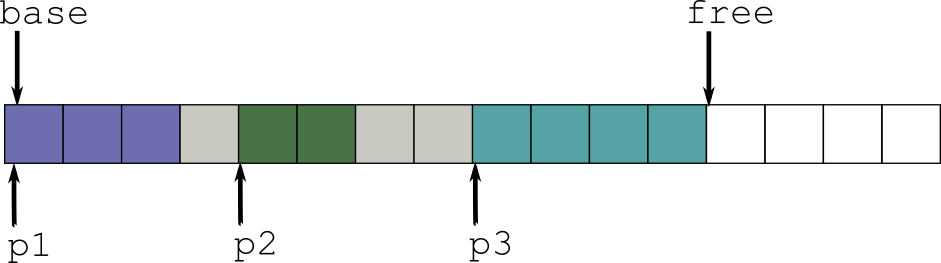
\includegraphics[width=.9\textwidth]{memgfx/monot_padding_020.png}
  \end{center}
\end{frame}


\begin{frame}[fragile]
  \frametitle{Monotonic Allocator - Extensions}
  \begin{center}
    \includegraphics<1-2>[width=.9\textwidth]{memgfx/monot_stack_010.png}
    \includegraphics<3>[width=.9\textwidth]{memgfx/monot_stack_020.png}
    \includegraphics<4-5>[width=.9\textwidth]{memgfx/monot_stack_021.png}
    \includegraphics<6>[width=.9\textwidth]{memgfx/monot_stack_030.png}
    \includegraphics<7>[width=.9\textwidth]{memgfx/monot_stack_040.png}
    \includegraphics<8>[width=.9\textwidth]{memgfx/monot_stack_050.png}
    \includegraphics<9>[width=.9\textwidth]{memgfx/monot_stack_060.png}
  \end{center}

  \begin{semiverbatim}
    \uncover<2->{\alert<2-3>{extpool.deallocate(p2);}}
    \uncover<5->{\alert<5-8>{extpool.deallocate(p3);}}
  \end{semiverbatim}
\end{frame}


\begin{frame}
  \frametitle{Monotonic Allocator - Extensions}
  \begin{itemize}
  \item Auxiliary data structure required
  \item Runtime cost of deallocation now linear in number of allocations (amortized O(1))
  \item Auxiliary nodes have their own alignment requirements
  \item Where to store the auxiliary nodes?
  \end{itemize}
\end{frame}

\begin{frame}[fragile]
  \frametitle{Monotonic Allocator - Extensions}
  \begin{center}
    \includegraphics<1>[width=.9\textwidth]{memgfx/monot_stack_010.png}
    \includegraphics<2>[width=.9\textwidth]{memgfx/monot_stack_external_010.png}
  \end{center}
\end{frame}


\begin{frame}
  \frametitle{Internal or External?}

  \begin{itemize}
  \item External headers have better cache behavior when iterating the list
  \item External headers might have stricter alignment requirements than data
  \item Internal headers have better cache behavior when adjacent data is hot
  \item Internal headers require managed memory to be readable (think GPUs)
  \item Where does the storage for external headers come from? Same buffer? Different buffer? How big?
  \end{itemize}
  
  $\Rightarrow$ No easy answers.
\end{frame}


\begin{frame}
  \frametitle{The Bottom Line\ldots}

  Even seemingly simple extensions get complicated very quickly.

  \vfill
  
  Don't try to increase generality through clever extensions.

  Only consider modifications if it's a perfect fit for your use case.
\end{frame}


\begin{frame}
  \frametitle{But what if I need to reclaim memory?}

  \vfill $\longrightarrow$ Pool Allocator \vfill
\end{frame}


\begin{frame}[fragile]
  \frametitle{Pool Allocator}
  \begin{center}
    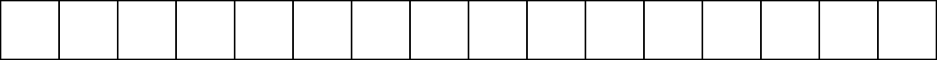
\includegraphics[width=.9\textwidth]{memgfx/empty.png}
  \end{center}
\end{frame}

\begin{frame}[fragile]
  \frametitle{Pool Allocator}
  \begin{center}
    \includegraphics<1>[width=.9\textwidth]{memgfx/pool_010.png}
    \includegraphics<2-3>[width=.9\textwidth]{memgfx/pool_020.png}
    \includegraphics<4>[width=.9\textwidth]{memgfx/pool_030.png}
    \includegraphics<5-6>[width=.9\textwidth]{memgfx/pool_040.png}
  \end{center}

  \begin{semiverbatim}
    \uncover<2->{\alert<2>{{\color{blue}auto} p1 = pool.allocate(2);}}
    \uncover<2->{\alert<2>{{\color{blue}auto} p2 = pool.allocate(4);}}
    \uncover<2->{\alert<2>{{\color{blue}auto} p3 = pool.allocate(3);}}
    
    \uncover<4->{\alert<4>{pool.deallocate(p1);}}
    \uncover<5->{\alert<5>{{\color{blue}auto} p4 = pool.allocate(1);}}
  \end{semiverbatim}
\end{frame}


\begin{frame}[fragile]
  \frametitle{Pool Allocator - Reclamation}
  \begin{center}
    \includegraphics<1>[width=.9\textwidth]{memgfx/pool_free_010.png}
    \includegraphics<2-3>[width=.9\textwidth]{memgfx/pool_free_020.png}
    \includegraphics<4>[width=.9\textwidth]{memgfx/pool_free_030.png}
    \includegraphics<5-6>[width=.9\textwidth]{memgfx/pool_free_040.png}
  \end{center}

  \begin{semiverbatim}
    \uncover<2->{\alert<2>{{\color{blue}auto} p1 = pool.allocate(2);}}
    \uncover<2->{\alert<2>{{\color{blue}auto} p2 = pool.allocate(4);}}
    
    \uncover<4->{\alert<4>{pool.deallocate(p1);}}
    \uncover<5->{\alert<5>{pool.deallocate(p2);}}
  \end{semiverbatim}
\end{frame}


\begin{frame}[fragile]
  \frametitle{Pool Allocator - Diffusion}
  \begin{center}
    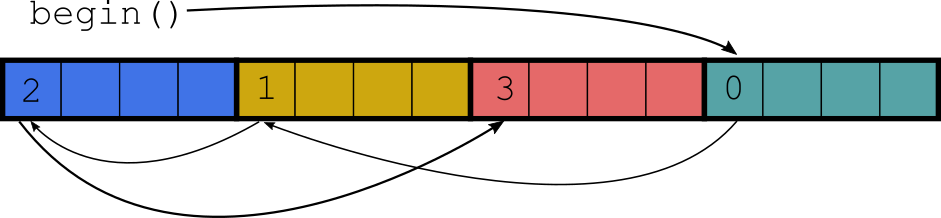
\includegraphics[width=.9\textwidth]{memgfx/pool_diffusion.png}
  \end{center}
\end{frame}


\begin{frame}[fragile]
  \frametitle{Pool Allocator}
  \begin{itemize}
  \item Deterministic runtime cost
  \item No external fragmentation
  \item Easy to make thread-safe
  \end{itemize}
  But:
  \begin{itemize}
  \item Cannot serve allocations bigger than chunk size
  \item High waste through internal fragmentation if sizes of objects vary a lot
  \end{itemize}
\end{frame}


\begin{frame}[fragile]
  \frametitle{Pool Allocator - STL containers}
  \begin{itemize}
  \item \texttt{vector} only if chunk sizes match vector size
  \item \texttt{list} and \texttt{map} perfect fit, as the size of each node is known beforehand (though this knowledge is implementation-specific)
  \item Similar for \texttt{deque}
  \item \texttt{unordered\_map} is again complicated
  \end{itemize}
\end{frame}


\begin{frame}
  \frametitle{But what if I do need different sizes?}

  \vfill $\longrightarrow$ Multipool Allocator \vfill
\end{frame}


\begin{frame}[fragile]
  \frametitle{Multipool Allocator}
  \begin{center}
    \includegraphics<1-2>[width=.9\textwidth]{memgfx/multipool_010.png}
    \includegraphics<3-4>[width=.9\textwidth]{memgfx/multipool_020.png}
    \includegraphics<5>[width=.9\textwidth]{memgfx/multipool_030.png}
  \end{center}

  \begin{semiverbatim}
    \uncover<2->{\alert<2>{{\color{blue}auto} p1 = multipool.allocate(6);}}
    \uncover<4->{\alert<4>{{\color{blue}auto} p2 = multipool.allocate(2);}}
  \end{semiverbatim}
\end{frame}


\begin{frame}[fragile]
  \frametitle{Multipool Allocator}
  \begin{itemize}
  \item Very powerful allocator
  \item Difficult to set up: How many pools do I need? What chunk sizes? What pool sizes?
  \item Solid building block for a general purpose allocator
  \end{itemize}
\end{frame}

\fi %crop


\begin{frame}[fragile]
  \frametitle{Allocator support in C++}

  \begin{semiverbatim}
std::vector<T, \alert<2>{Allocator<T>}> v;
    
v.push\_back(\ldots);
  \end{semiverbatim}

  \uncover<2->{This is not the class allocating the memory.}
\end{frame}


\begin{frame}[fragile]
  \frametitle{Allocator support in C++}

  Historically, allocators in C++ were a way to abstract different models of addressing memory.

  As such, \textit{Allocators} in C++ are ``stateless''.  \\~\

  \pause
  \alert<2>{In C++ an Allocator is merely a handle to a \textit{memory resource}.}\footnote{\href{https://www.youtube.com/watch?v=0MdSJsCTRkY}{Arthur O'Dwyer - An Allocator is a Handle to the Heap}}
\end{frame}


\begin{frame}[fragile]
  \frametitle{Allocator support in C++}

  \begin{semiverbatim}
std::pmr::memory\_resource& mr = \ldots;
\uncover<1-3>{std::vector<T, \alert<2>{std::pmr::polymorphic\_allocator}> v(\alert<3>{&mr});}
\uncover<4>{\alert<4>{std::pmr::vector<T> v(\alert<3>{&mr});}}
    
v.push\_back(\ldots);
  \end{semiverbatim}

  \begin{itemize}
    \uncover<2->{\item Enable custom allocators for the object.}
    \uncover<3->{\item Pass a \texttt{memory\_resource} to handle allocation/deallocation.}
  \end{itemize}
\end{frame}


\begin{frame}[fragile]
  \frametitle{C++ Memory Resources\footnote{\href{https://www.youtube.com/watch?v=v3dz-AKOVL8}{Pablo Halpern - Allocators: The Good Parts}}}

  \begin{itemize}
  \item \texttt{std::pmr::memory\_resource} - Abstract base class for all resources consumable by \texttt{std::pmr::polymorphic\_allocator}
  \item \texttt{std::pmr::new\_delete\_resource} - Global allocator
  \item \texttt{std::pmr::monotonic\_buffer\_resource} - Monotonic allocator
  \item \texttt{std::pmr::unsynchronized\_pool\_resource}/ \texttt{synchronized\_pool\_resource} - Multipool
  \item \texttt{std::pmr::null\_memory\_resource} - Allocation always fails
  \end{itemize}
\end{frame}


\begin{frame}[fragile]
  \frametitle{Chaining}
  \begin{lstlisting}
explicit monotonic_buffer_resource(
  std::pmr::memory_resource* upstream);
  \end{lstlisting}

  Each \texttt{memory\_resource} has an upstream counterpart. \\~\

  If the resource runs out of memory, it tries to allocate more memory from upstream.
\end{frame}


\begin{frame}[fragile]
  \frametitle{Chaining}
  Possible uses of Chaining:
  \begin{itemize}
  \item Fixed-size vs. dynamic storage for allocators
  \item Combination of different allocation strategies
  \item Injection points for special purpose allocators for debugging and profiling
  \end{itemize}
\end{frame}


\begin{frame}
  \frametitle{There's no universal interface for allocators}

  \begin{itemize}
  \item Are size and alignment parameters passed to \texttt{deallocate}?
  \item Is \texttt{realloc} supported?
  \item How are out-of-memory errors reported?
  \item Is extended alignment supported?
  \item What is the return value for an allocation of size \texttt{0}?
  \item Different memory regions for internal data structures and allocated memory?
  \end{itemize}
\end{frame}


\begin{frame}
  \frametitle{Don't underestimate the global allocator}

  \begin{itemize}
  \item Competitive performance in the general case
  \item Security features (ASLR, secure erase of freed memory)
  \item Debugging \& Profiling (Valgrind, Windows Debug Runtime)
  \item Cache Coloring
  \end{itemize}

  Local allocators are no free lunch!
\end{frame}


% c++ allocator model: handle to the heap, stateful vs stateless
% pmr memory resource
% chaining; debug allocators
% differences between allocator implementations

\iffalse
\begin{frame}[fragile]
  \frametitle{Let's talk about memory}
    \begin{itemize}
    \item Dynamic memory: Request objects using allocate, deallocate to give memory back
    \item Done! Or is it?
    \end{itemize}
    Problems with global allocator:
    \begin{itemize}
    \item No one-size fits all allocation strategy. Every allocator has an achilles heel.
    \item Global allocators don't parallelize well. Allocation/Deallocation typically requires acquiring a lock.
    \item Runtime performance of global allocators is unpredictable. Understanding runtime behaviour requires understanding the entire program
    \item Overhead of the allocation algorithm might not be acceptable on the target hardware.
    \end{itemize}
\end{frame}

\begin{frame}[fragile]
  \frametitle{Main concerns about dynamic memory}
    \begin{itemize}
    \item Maximum overall memory consumption.
    \item Runtime behavior.
    \item Fragmentation.
    \end{itemize}
\end{frame}

\begin{frame}[fragile]
  \frametitle{Local allocators to the rescue}
    Pro:
    \begin{itemize}
    \item 
    \end{itemize}

    Con:
    \begin{itemize}
    \item Allocating memory requires access to an allocator.
    \end{itemize}
\end{frame}
\fi

\begin{frame}
  \frametitle{Thanks for your attention.}
\end{frame}


\end{document}
